% This file was created by matlab2tikz.
%
%The latest updates can be retrieved from
%  http://www.mathworks.com/matlabcentral/fileexchange/22022-matlab2tikz-matlab2tikz
%where you can also make suggestions and rate matlab2tikz.
%
\documentclass[tikz]{standalone}
\usepackage[T1]{fontenc}
\usepackage[utf8]{inputenc}
\usepackage{pgfplots}
\usepackage{grffile}
\pgfplotsset{compat=newest}
\usetikzlibrary{plotmarks}
\usepgfplotslibrary{patchplots}
\usepackage{amsmath}

\begin{document}
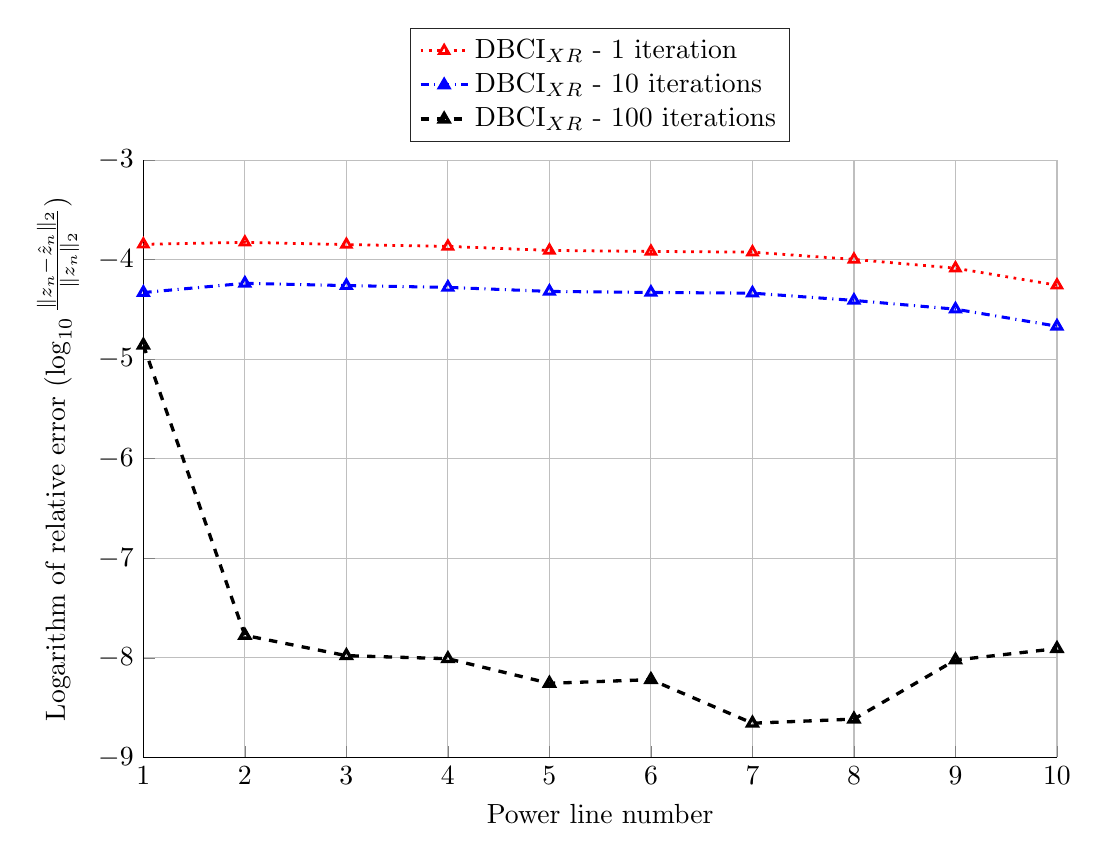
\begin{tikzpicture}

\begin{axis}[%
width=4.568in,
height=2.986in,
at={(0.766in,0.427in)},
scale only axis,
xmin=1,
xmax=10,
xlabel={Power line number},
xmajorgrids,
ymin=-9,
ymax=-3,
ylabel={Logarithm of relative error ($\log_{10}\frac{\|z_n - \hat{z}_n\|_2}{\|z_n\|_2}$)},
ymajorgrids,
axis background/.style={fill=white},
axis x line*=bottom,
axis y line*=left,
legend style={at={(0.5,1.03)},anchor=south,legend cell align=left,align=left,draw=white!15!black}
]
\addplot [color=red,dotted,line width=1.0pt,mark=triangle,mark options={solid}]
  table[row sep=crcr]{%
1	-3.84566886657509\\
2	-3.82565119072312\\
3	-3.84833128896708\\
4	-3.86623240670023\\
5	-3.90703903414787\\
6	-3.91725298355195\\
7	-3.9242906832263\\
8	-3.99755447774431\\
9	-4.0854130784046\\
10	-4.25639565924659\\
};
\addlegendentry{DBCI$_{XR}$ - 1 iteration};

\addplot [color=blue,dashdotted,line width=1.1pt,mark=triangle,mark options={solid}]
  table[row sep=crcr]{%
1	-4.33000124603526\\
2	-4.23754131023292\\
3	-4.26024115528396\\
4	-4.27813879543128\\
5	-4.31895353102911\\
6	-4.32916144447768\\
7	-4.33621901699141\\
8	-4.40946293264974\\
9	-4.49724263354282\\
10	-4.66843483824481\\
};
\addlegendentry{DBCI$_{XR}$ - 10 iterations};

\addplot [color=black,dashed,line width=1.2pt,mark=triangle,mark options={solid}]
  table[row sep=crcr]{%
1	-4.85887380114855\\
2	-7.77460579190817\\
3	-7.97834380289756\\
4	-8.00916693173165\\
5	-8.25638146026475\\
6	-8.2193017540687\\
7	-8.65707562049412\\
8	-8.61586947063308\\
9	-8.02222749870226\\
10	-7.90759695306159\\
};
\addlegendentry{DBCI$_{XR}$ - 100 iterations};

\end{axis}
\end{tikzpicture}%
\end{document}